\section{Metod} 

Nedan följer en beskrivning av de arbetsmetoder vi använt oss utav och de mjukvaror och kodbibliotek som vi använt oss utav i projektet. 

\subsection{Arbetsmetodik}

% modulbaserat arbete..
Under planeringsstadiet upptäcktes tidigt att projektet kunde med delas upp i tre separata moduler; parser, interpretator och typcheckare. Dessa tre moduler intergrerar enbart med varandra genom det abstrakta syntaxträdet. Detta medför att det är väldigt lätt att utveckla de olika delarna helt frånskilt från varandra. Figur 1 visar hur denna interaktion mellan de olika modulerna är tänkt att gå till. Man ser även att webbläsaren kommunicerar genom ett Javascript API och det abstrakta syntaxträdet och inte direkt med de olika komponenterna. 

\begin{figure}[H]
    \begin{center}
        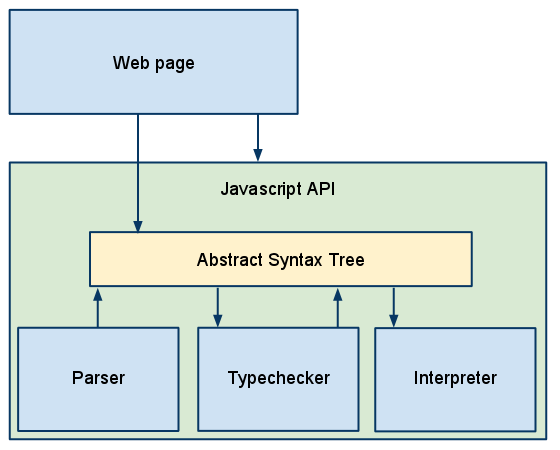
\includegraphics[width=1.0\textwidth]{image1.png}
        \caption{Överblick över tolkens struktur och interaktion}
    \end{center}
\end{figure}


Arbetssättet präglades utav en iterativ utvecklingsmetodik med korta utvecklingscyklar. Arbetet delades upp med huvudansvarstagande över var sin modul. Arbetet skedde dock framförallt i samlad grupp för att snabbt kunna delge information om vad som behövde implementeras för att samverkan mellan de olika modulerna skulle fungera friktionsfritt.

\subsection{Kodstandard} 
För att få konsistens i koden och för att underlätta att olika utvecklare kan läsa och arbeta på koden samtidigt har vi utformat en intärn kodstandard som alla ska följa.
När en commit görs måste denna standard följas.
% MOOOAARRR!! 

\subsection{Versionshantering} 
Ett problem som alla mjukvaruprojekt av icke trivial storlek är att hantera den stora mängden filer, och distrubera uppdaterade kopior till samtliga utvecklare att arbeta på.
För att lösa detta problemet brukar man använda sig utav en versionshanteringsmjukvara. 

Under de första veckorna av projektet användes SVN. Valet berodde på att  alla medlemmar i projektet hade erfarenhet från det tidigare. Tyvärr har SVN vissa problem när det kommer till att skapa nya förgreningar och sammanfoga dem. Därför gick valet till att använda sig utav Git. Git är designat från grunden för att på ett enkelt sätt skapa nya och slå samman förgreningar under utvecklingens gång. Vi kunde därmed skapa en förgrening för varje modul och under arbetets gång sammanlänka allas arbeten på ett effektivt sätt. 

\subsection{Javascript} 
Javascript \citep{javascript} är ett programmeringsspråk som framförallt används på klientsidan på webben. Javascript är ett dynamiskt objektorienterat skriptspråk.
Javascript är det programmeringsspråk som används uteslutande i detta projektet.

\subsection{Kodbibliotek}

\emph{Standing on the Shoulder of Giants}

Detta projektet följer en fin tradition inom datorvetenskapen att om ett problem redan är löst så ska det inte behöva lösas igen. Att återuppfinna hjulet varje gång är både tidsödande och onödigt. 
Därför har ett antal kodbibliotek används i projektet. 
Genom att använda dessa kodbibliotek kan fokus läggas på implementeringen av de kärnområden som projektet behandlar.
Nedan följer en kort beskrivning av de olika kodbibliotek som vi använt i projektet.

\subsubsection{JSParse}  
Parsern implementeras med hjälp av ett parser combinator bibliotek kallat JSParse. 
En parser combinator består av olika funktioner som parsar exempelvis strängar, listor och blanksteg. Dessa funktioner kombineras för att skapa mer komplexa parsers. JSParse ger oss möjlighet att enkelt implementera både den kontextfria och den del som inte är det av Haskells syntax.

\subsubsection{jQuery} 

jQuery är ett öppet kodbibliotek till Javascript som är dubeellicenserat under MIT License och GPL version 2.  
jQuery är designat för att underlätta för utvecklare att modifiera DOM-träd, HTML, och göra asynkrona javascript-anrop.

jQuery används i projektet för att få enkelt cross browser stöd utan att behöva tänka på det. 
jQuery ger även möjlighet att skapa ett enkelt och stilrent interaktivt gränssnitt utan att behöva göra allt från grunden.
Ett tillägg till jQuery kallat jQuery.Cookie används även för att förenkla användandet utav kakor.
